% reducesymm/blog/dailyBlogBB.tex
% $Author$ $Date$
% Predrag  switched to github.com               jul  8 2013
% continues siminos/blog/dailyBlog.tex as of that date

\chapter{Burak's daily blog}
\label{c-dailyBlogBB}

\renewcommand{\LieEl}{\ensuremath{g}}  % Predrag Lie group element
\renewcommand{\gSpace}{\ensuremath{\theta}}   % group rotation parameters
\renewcommand{\ssp}{x}
\renewcommand{\sspRed}{\ensuremath{\hat{x}}}  % reduced state space point
\renewcommand{\vel}{\ensuremath{v}}   % state space velocity

\begin{description}
\item[2013-07-11  Predrag to Burak] The last common entry with the svn repository \texttt{siminos/blog/dailyBlog.tex} is

{\bf [2013-03-14 Evangelos]} In
\emph{Quasiperiodic oscillations and homoclinic orbits in the nonlinear nonlocal
Schr\"odinger equation}, \arXiv{1303.3213}...

then the two blogs diverge. This file
\texttt{reducesymm/blog/dailyBlogBB.tex}
has only Burak work; do not edit anything in
the older \texttt{reducesymm/blog/dailyBlog.tex}

\item[2013-07-07  Predrag]
Burak (Nazmi B. Budanur <burakbudanur@gmail.com>), a new theory graduate student, started at GaTech Aug 2013, is joining us. He will focus on slicing, hopefully
slicing for pipe flows.

\item[2013-07-11  Predrag to Burak]
A better version of today's tutorial:
\HREF{http://chaosbook.org/~predrag/papers/WHole12.pdf} {8 Aug 2012 talk}.

Read \HREF{http://www.cns.gatech.edu/~predrag/papers/preprints.html\#atlas12} {Cvitanovi\'c \etal} \emph{Cartography of high-dimensional flows: A visual guide to sections and slices}\rf{atlas12}, blog here about things you understand or do not understand.

\item[2013-07-12  Burak] I started feeling lost in section IV of the
    paper. I think I should work on simpler examples of Poincar\'e
    sections and method of slices to make the distinction well. For
    that purpose, I thought about going through examples of Chapter III
    of ChaosBook and then trying to reproduce
    \HREF{http://www.cns.gatech.edu/~predrag/papers/FrCv11.pdf}
    {Froehlich \& Cvitanovi\'c} \emph{Reduction of continuous
    symmetries of chaotic flows by the method of slices}\rf{FrCv11}. Is
    this a good idea?

\item[2013-07-12  Predrag] I would go through
\wwwcb{/paper.shtml\#maps} {\em Chapter  - Discrete time dynamics} examples first, then
we think of the next step?

\item[2013-07-12  Burak]
I did not get an e-mail notification after your commit yesterday and I found out that it is not default in github.

To get notifications for commits, under
\begin{verbatim}
Settings -> Service Hooks -> E-mail
\end{verbatim}
You should enter e-mails that we want the notifications to be sent.

I checked this on one of my repository and it works.

What is annoying is, we can only enter two e-mail addresses in this area, which is not a problem right now but it will be when others join github. To work this around, I can set up a ``forwarder" e-mail address for the project which would forward the e-mails that it receives to the participants of the project so that everyone can be notified.
\item[2013-07-12  Predrag] Check whether paid accounts have unlimited email lists (I seem to remember that bitBucket free accounts were up to 5 collaborators). I
    do not mind paying from a grant, if the thing works...

\item[2013-07-15  Burak]
I talked to the github support and learned that they do not send notifications for pushes. I then checked Bitbucket (github clone), setting up e-mail notifications is pretty similar:
\begin{verbatim}
Settings -> Services -> E-mail->Add service
\end{verbatim}
As you said, we are also able to get private repositories with up to 5 collaborators on Bitbucket.

It is also possible to workaround this problem on github by starting a mail list and setting that up such that it forwards mails it recieves from github to the people on the list.

\item[2013-07-15  Burak]
I have done most of the exercises 2.8, 3.1, 3.2, 3.7 (ChaosBook
version14.4.1) and re-read the paper.

In exercise 3.2 what exactly do you mean by ``Euclidean length s
computed curvilinearly along the attractor section''? Is it the
distance along the orbit?
\item[2013-07-18  Predrag] Read
Section 12.1.1 {\em Parametrization of invariant manifolds}. I've now
included link to this section in exercise 3.2 {\em A return Poincar\'e map for the R\"ossler flow.}

\item[2013-07-15  Burak]
Another question about
\HREF{http://www.cns.gatech.edu/~predrag/papers/preprints.html\#atlas12}
{Cvitanovi\'c \etal} \emph{Cartography of high-dimensional flows: A
visual guide to sections and slices}\rf{atlas12}. How do you get the
tangent vector in the extremum condition, eqs.~(6), (7). I would
understand it if the transformation was infinitesimal but I do not see
it for $\gSpace$ from 0 to $2 \pi$.
\item[2013-07-18  Predrag]
We discussed it today - can you write down the answer here?

\item[2013-07-21  Burak] In the equation, $\sspRed$ is $\ssp$,
    transformed like $\sspRed = \LieEl^{-1}(\gSpace) \ssp$ such that it is closest
    to the template point $\slicep$. Now, it does geometrically make
    sense to me that the extremum condition should require that vectors
    $(\sspRed - \slicep)$ and $ \sliceTan{} = \Lg \slicep$ to be
    perpendicular to each other, however, I still am not able to show
    this algebraically by just taking the derivative with respect to
    $\gSpace$.
\item[2013-07-22  Predrag] Bummer, read
    \HREF{http://chaosbook.org/paper.shtml\#continuous} {Chapter 10} -
    {\em Relativity for cyclists} very critically, I have to rewrite
discussion of slicing (still have not described the extremal distance
condition). Please reread the argument in Froehlich \&
Cvitanovi\'c\rf{FrCv11}, if it now makes sense to you, summarize the
argument here, with an eye on having me update this in ChaosBook...

\item[2013-07-15  Burak] Going through
    \HREF{http://chaosbook.org/paper.shtml\#maps} {Chapter 3} and
    examples was really helpful, should I continue with
    \HREF{http://chaosbook.org/paper.shtml\#continuous} {Chapter 10} -
    {\em Relativity for cyclists} \&
    \HREF{http://chaosbook.org/paper.shtml\#knead} {Chapter 11} -
    {\em Charting the state space?}
\item[2013-07-18  Predrag]
We discussed it today - enter the plan here?

\item[2013-07-21  Burak] The current plan is, before Chapter 10, I will
    finish  \HREF{http://chaosbook.org/paper.shtml\#discrete} {Chapter
    9} - {\em World in a mirror} and after going through Chapter 10 and
    11, I will have a look at the Porter-Knobloch blog and try to find
    parameters that can make the equations behave chaotic.

\item[2013-07-23  Burak] Question on the derivation of eq. (10.51) of \HREF{http://chaosbook.org/paper.shtml\#continuous} {Chapter 10} - {\em Relativity for cyclists}: We have the slice condition:
\beq
 \sspRed^T \sliceTan{a} = 0.
\eeq
Substituting (10.49), I would have written down its time derivative as
\beq
 \velRed^T \sliceTan{a} = v(\sspRed)^T \sliceTan{a} - \dot{\phi}(\sspRed) \cdot t(\sspRed)^T \sliceTan{a}=0.
\eeq
However, this, in ChaosBook, is written as
\beq
 \velRed^T \sliceTan{a} = v(\sspRed)^T \sliceTan{a} - \dot{\phi_a}(\sspRed) \cdot t(\sspRed)^T \sliceTan{a}=0.
\eeq
I thought, $\phi \cdot \groupTan$ meant $\phi_1 t_1 + \phi_2 t_2 + \phi_3 t_3 + ... $ is this accurate? If so, dot product of a particular $\phi_a$ with $t(\sspRed)^T$ doesn't make sense to me. You also drop the indice a from the template tangent vector on the denominator of 10.51 and write it as dot product of tangent at x and the template tangent. I cannot see this
as well.

\item[2013-07-24  Predrag]
You poked your finger into a painful spot - We have used the
slicing condition only on Abelian cases such as $\SOn(2)$ and
$\SOn(2)\times\SOn(2)$, and I had never derived the correct formula for
non-Abelian case.

See
{\bf [2011-07-08 PC]} above (currently p.~89)
{\bf [2011-07-08 Predrag]} above (currently p.~115).
Someplace (in Froehlich?) we say that we would have to invert a matrix in
the general case - anyway, my formula is probably wrong, try to do it
your own way. Git pushing all figures for atlas12.tex paper now, might
continue on this later.

\item[2013-07-25  Predrag] (continued). Here is what we write in
\refref{FrCv11}, Sect.~{\em Dynamics within a slice}:
%\label{sec:mslices}

Any \statesp\ trajectory can be written in a factorized
form $\ssp(\tau)=\LieEl(\tau)\,\sspRed(\tau)$
(here $\LieEl(\tau)$ is a shorthand for $\LieEl(\gSpace(\tau))$,
or perhaps even $\LieEl(\gSpace(\ssp(\tau)))$).
Differentiating both sides with respect to time and
setting $\velRed={d\sspRed}/{d\tau}$ we find
\(
\vel(\ssp)=\dot{\LieEl} \, \sspRed+\LieEl \, \velRed(\sspRed)
\,.
\)
By the equivariance %\refeq{eq:FiniteRot}
\[
\vel(\sspRed)=\velRed(\sspRed) + \LieEl^{-1} \, \dot{\LieEl} \, \sspRed
\,.
\]
Noting that $\LieEl^{-1}\dot{\LieEl}=e^{-\gSpace \cdot \Lg} \,
\frac{d ~~}{d \, \tau} e^{\gSpace \cdot \Lg}=\dot{\gSpace}\cdot \Lg$,
we obtain the equation for the velocity of the reduced flow:
\beq
\velRed(\sspRed)=\vel(\sspRed)-\dot{\gSpace}(\sspRed)\cdot \groupTan(\sspRed)
\,.
\ee{eq:redVel}
The velocity $\vel$ in the full \statesp\ is thus the sum of the
`phase' velocity %\refeq{PC:groupTan1}
along the group orbit, $\dot{\gSpace} \cdot \groupTan(\sspRed)$,
and the remainder $\velRed$.

Eq. \refeq{eq:redVel} is true for any factorization
$\ssp=\LieEl \sspRed$, and by itself provides no
information on how to calculate $\dot{\gSpace}$. That is attained by
demanding that the reduced trajectory stays within a slice, by imposing
the slice conditions: % \refeq{PCsectQ}:
% PC 2013-07-25 added 2. equation
\bea
       \braket{\dot{\gSpace}\cdot \groupTan(\sspRed)}{\sliceTan{a}}
 &=& \braket{\vel(\sspRed)}{\sliceTan{a}}
    \continue
\sum_b \dot{\gSpace}_b \braket{ \groupTan{}_b(\sspRed)}{\sliceTan{a}}
 &=&
\braket{\vel(\sspRed)}{\sliceTan{a}}
\,.
\label{eq:slicecondition}
\eea
This is a matrix equation for the $N$\dmn\ vector $\dot{\gSpace}_b$ solved
by inverting the \statesp\ position dependent matrix
$\braket{\groupTan_b(\sspRed)}{\sliceTan{a}}$.
We consider here only the
$\SOn{2}$ case, which has a single group tangent:
\bea
\velRed(\sspRed) &=& \vel(\sspRed)
   -\dot{\gSpace}(\sspRed) \, \groupTan(\sspRed)
\continue
\dot{\gSpace}(\sspRed) &=& {\braket{\vel(\sspRed)}{\sliceTan{}}}/
               {\braket{\groupTan(\sspRed)}{\sliceTan{}}}
\,.
\label{eq:so2reduced}
\eea
One way to think about this reduction of a flow to a slice is in terms of
Lagrange multipliers (see {Stone and Goldbart}\rf{StGo09}, Sect 1.5 for
intuitive, geometrical interpretation of Lagrange multipliers). The first
equation defines the flow confined to the slice,
the `shape', `template' or `slice' dynamics\rf{rowley_reduction_2003},
% (see \reffig{fig:Fullspace}\,(b), \reffig{fig:slice}\,(a)),
and integration of the second,
`reconstruction' equation\rf{Marsd92,MarsdRat94} enables us to track the
corresponding trajectory in the full \statesp. For invariant subspaces
$\dot{\gSpace}=0$, so they are always included within the slice. No
information is lost about the physical flow: if we know one point on a
trajectory, we can hop at will back and forth between the reduced
and the full \statesp\ trajectories, just as we can reconstruct a
continuous trajectory from its \PoincSec s.

\item[2013-07-25  Predrag]
The authors of \refrefs{ahuja_template-based_2007,FiSaScWu96} claim one
can in principle solve equation \refeq{eq:so2reduced} for any Lie group.
\refRef{FiSaScWu96} does not do it. Ahuja does not either.... If go to a
nonabelian symmetry such as \SOn{3} or \SUn{2} I think we will have to
solve this numerically.

\item[2013-07-25  Predrag] as the matrix
$\braket{\groupTan_b(\sspRed)}{\sliceTan{a}}$ depends on a product of
two Lie group representations,
\beq
\braket{\groupTan_b(\sspRed)}{\sliceTan{a}}
 =
 - \sspRed_i \slicep_j \Lg^b_{k\ell}\Lg^a_{\ell j}
\,,
\label{eq:so2reduced}
\eeq
for a particular group this can be expressed as a Kronecker sum of
irreducible representations. Have not tried that.

\item[2013-07-25  Burak]
I finished \HREF{http://chaosbook.org/paper.shtml\#continuous} {Chapter
10} - {\em Relativity for cyclists} yesterday. I'm summarizing my
understanding: \Reducedsp\ is useful for visualization because on
the slice, \rpo s become \po s. It
is more useful than co-moving frames method, because with co-moving
frames you can only catch one relative orbit or maybe it's integer
dividers, but in method of slices you get them all (There may be a
stronger reason, this is what I understood for now). We can implement
the slice method in two different ways: Method of moving frames
(post-processing) and dynamics within the slice.

In the moving frames method, we take a full solution (a numerical
simulation or experimental data), and pick a slice hyperplane (a hyperplane
given by $\langle \sspRed - \slicep | \sliceTan{} \rangle = 0$ where
point $\slicep$ is called a template, and $\sliceTan{} = \Lg  \slicep$ is
the group tangent at the template point) and find the transformations
$\sspRed(\tau) = g(\phi(\tau))^{-1} \ssp(\tau)$ which satisfies the slice
condition. For \SOn{n}, infinitesimal generator \Lg\  is antisymmetric
hence the template tangent is perpendicular to template point, and the
slice condition simplifies to $\langle \sspRed | \sliceTan{} \rangle =
0$. Getting the point $x$ to the slice hyperplane by group operations
would be equivalent to the minimizing the Euclidian distance between the
transformed point and the template point because by doing that, we
eliminate the distance between points $\sspRed$ and $\slicep$
perpendicular to the slice hyperplane and only remaining separation is
the separation on the slice.
    \BB{2012-07-25}
    {Is this a correct way of understanding the extremum argument? {\bf
    Predrag} There are at least two solutions (the closest, the most
    distant) to the slice condition, and in general, many more. So you
    need to write up a discussion along the lines of \refref{atlas12}, a
    local copy, with all internal comments is \HREF{../atlas/atlas12.pdf}
    {here}. One has to be precise about the language - definitions are given
    in Sect.~\emph{V. Charting the slice}.
    }
Here are
the resulting plots my attempt of applying moving frames method on
\cLf:

\begin{figure}[ht]
\begin{center}
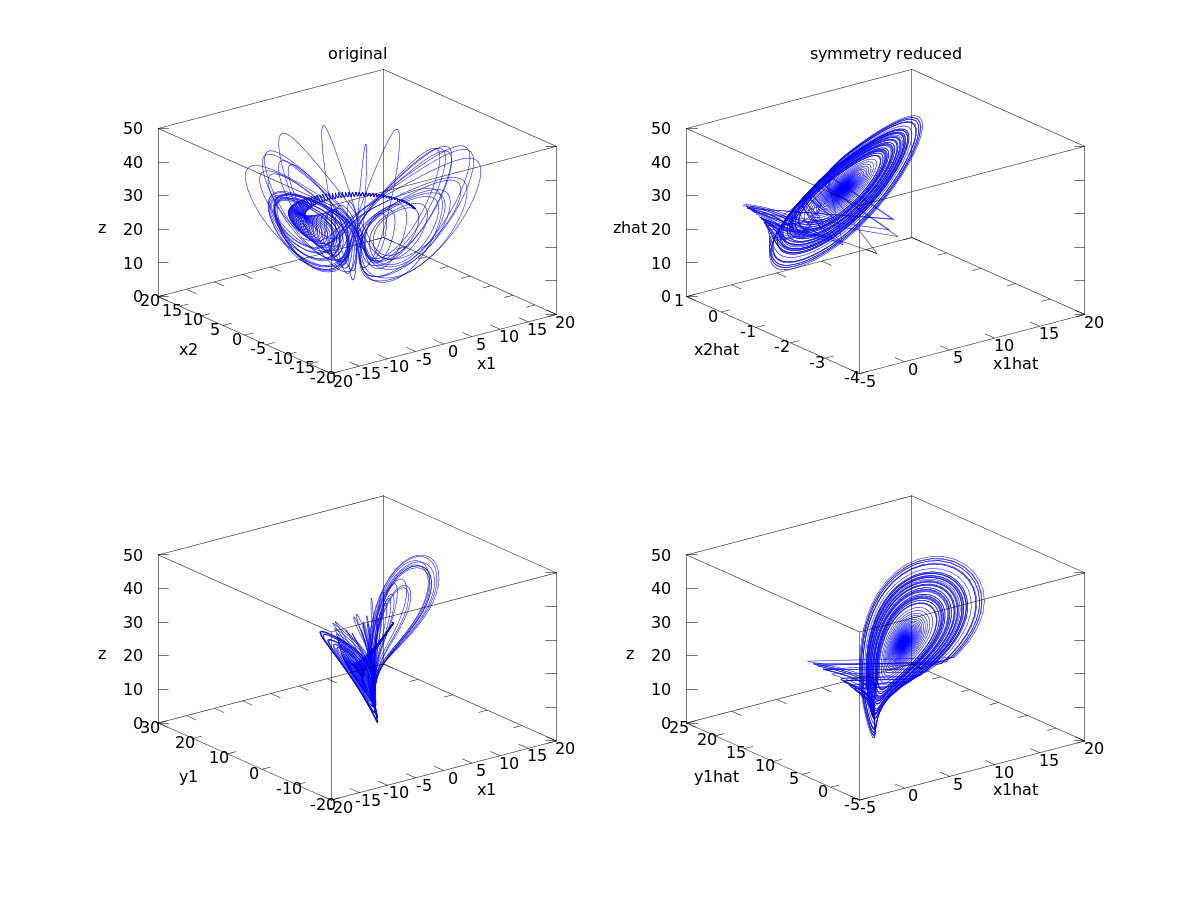
\includegraphics[width=0.9\textwidth]{BBmovingframes}
\end{center}
\caption{ Method of moving frames applied on \cLf.
    }
\label{fig:BBmovingframesCL}
\end{figure}

We can, at least when the symmetry group is abelian, solve the dynamics
on the \reducedsp\ and after that, map it back to the full \statesp\ if
we want to. For the dynamics within the slice, \SOn{2} symmetry we get following
equations:
\bea
  \velRed(\sspRed) &=& \vel(\sspRed) - \dot{\phi} (\sspRed) \groupTan(\sspRed)
\continue
  \dot{\phi}(\sspRed)
    &=& \braket{\vel(\sspRed)}{\sliceTan{}}
    / \braket{\groupTan(\sspRed)}{\sliceTan{}}
\,.
\eea
Here the problem is possibility of getting tangent at the point
$t(\sspRed)$ and the template tangent perpendicular to each other. For
this reason we need multiple, intersecting charts in such a way that this
does not happen. Then we can solve the problem on the
\reducedsp. My unsuccessful attempt of solving reduced dynamics on one
slice:

\begin{figure}[ht]
\begin{center}
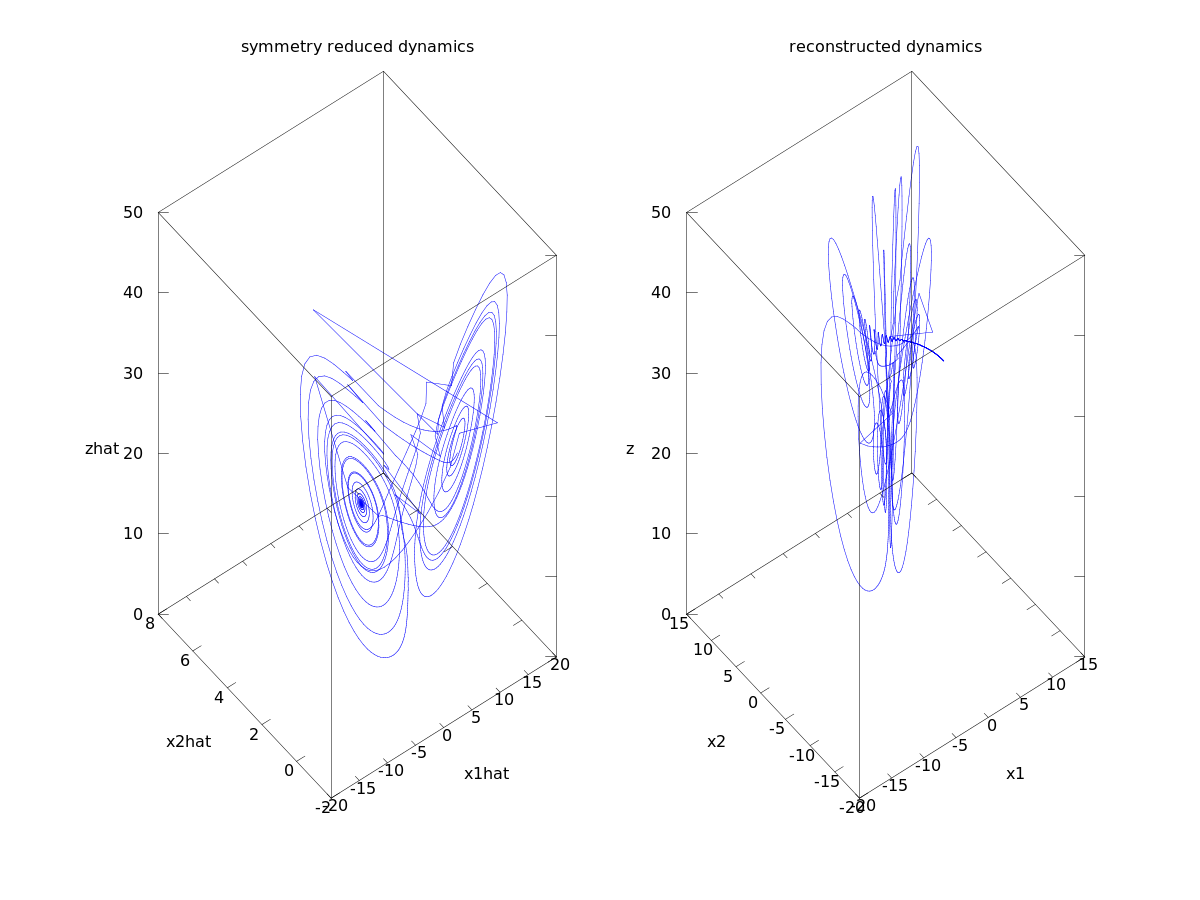
\includegraphics[width=0.9\textwidth]{BBslicedynamics}
\end{center}
\caption{ Dynamics of \cLf\ computed on one slice.
    }
\label{fig:BBslicedynamics}
\end{figure}

\item[2013-07-25  Predrag]
I have edited your formulas using our macros - it does not matter right
now, but it will be handy later, as one uses different notation for ODE
and PDE \statesp s, for example. One has to be precise about the
language, otherwise one ends up with several things being called `slice',
for example. Definitions are given in Sect.~\emph{V. Charting the slice}
of \refref{atlas12}. A local copy, with all internal comments, is
\HREF{../atlas/atlas12.pdf} {here}.

\refFig{fig:BBmovingframesCL} and \reffig{fig:BBslicedynamics} look
a bit buggy, but basically right.

\item[2013-08-10  Predrag] Moved all Burak's
\twoMode\ $\SOn{2}$-equivariant flow experimentation to file
\texttt{siminos/blog/2modesBB.tex}.

\item[2013-09-10 Burak] I might have found a general way of reducing the symmetry using single slice:

Let us have an m-mode $\SOn{2}$-equivariant system with the Lie algebra generator
\beq
	\Lg =  \begin{pmatrix}
			 0  & 1 & 0 & 0 & \cdots & 0 & 0\\
			 -1 & 0 & 0 & 0 & \cdots & 0 & 0\\
			 0  & 0 & 0 & 2 & \cdots & 0 & 0\\
			 0 & 0 & -2 & 0 & \cdots & 0 & 0\\
			 \vdots  & \vdots  & \vdots  & \vdots  & \ddots & \vdots & \vdots  \\
			 0 & 0 & 0 & 0 & \cdots & 0 & m \\
			 0 & 0 & 0 & 0 & \cdots & -m & 0
			\end{pmatrix} .
	\label{eq:LgSO2}
\,.
\eeq
Let $\slicep$ be a \slice\ template and  $\sspRed^{*}$ be a point on its \chartBord. In this general case, \chartBord\ conditions \refeq{eq:chartBord} reads:
\begin{subequations}\label{eq:mmodechartbord}
\begin{align}
	\sum_{k=1}^{m} k  (\sspRed_{2k-1}^{*} \slicep_{2k} - \sspRed_{2k}^{*} \slicep_{2k-1})&= 0 ,
	\label{eq:mmodechartborda}
\\
	\sum_{k=1}^{m} k^2 (\sspRed_{2k-1}^{*} \slicep_{2k-1} + \sspRed_{2k}^{*} \slicep_{2k}) &= 0
	\label{eq:mmodechartbordb} .
\,
\end{align}
\end{subequations}
Where subscripts denots vector components. For the particular choice of $\slicep=\{1,1,0,0,\cdots,0\}$ equations \refeq{eq:mmodechartbord} reduces to:
\begin{subequations}\label{eq:mmodechartbordred}
\begin{align}
	\sspRed_{1}^{*} - \sspRed_{2}^{*} &= 0 ,
	\label{eq:mmodechartbordreda}
\\
	\sspRed_{1}^{*} + \sspRed_{2}^{*} &= 0 .
	\label{eq:mmodechartbordredb}
\,
\end{align}
\end{subequations}
Which is only solved if $\sspRed_{1}^{*} = \sspRed_{2}^{*} = 0$.
Thus, it is possible to reduce the symmetry of an $m$-mode $\SOn{2}$-equivariant 
system using the single template point $\slicep=\{1,1,0,0,\cdots,0\}$ if 
the amplitudes of the first Fourier mode of the system never simultaneously vanish.

\item[2013-09-11 Predrag] This, I think, is the first thing we tried,
and what Ruslan believes is the solution, so he has since refused any of
the slicing entanglements that we have developed.
He might well be right - I would love the simplest solution to be the
right one. Read
\refsect{2008-01-17How2QuotientSO2},
\refsect{2009-08-25Eurosceptics},
\refsect{2009-08-29KS-O2} and so on. Please read those discussions critically.
We did not follow Ruslan's prescription, right or wrong.

At some point, you might want to read / scan through
all 300+ pages of the historical blog, ask me
questions if anything looks different.

\item[2013-09-11 Daniel] So where are we blogging now? Seems like
stuff is getting moved all over the place... Anyway, while I don't
immediately see an error in Burak's logic, the figure of a single
slice based on the the template (1,1,1,1,0) for \cLf\, seems odd.
When I run my code, I basically get something like figure 4c in the
atlas paper. I haven't run it in a long time so MAYBE I'm doing it
wrong but I think I'm doing it right. Will double check. Looking at
the phase velocity, I get that it gets huge ($\sim$1000). We also
know what the symmetry reduced attractor should look like since
Siminos has studied it in a Hilbert invariant polynomial basis (as
shown in section 10.5 of Das Buch). Both of these things are
single-lobed (with the single-sliced attractor having some
discontinuities), but your figure shows a two-lobed thing. I think
that at one point, we discussed the fact that in the case of \cLf,
just getting to close to the z axis makes the phase velocity blow up,
i.e., you don't actually have to reach the chart border. My
hypothesis at the time was that my cooked up templates for the two
slice atlas worked because they just happened to keep you away from
the z axis as much as possible. That discussion is probably buried
somewhere in the atlas blog.

\item[2013-09-11 Predrag]
\texttt{reducesymm/cgang/2modes.tex} is specific to \twoMode\ article,
\texttt{reducesymm/blog/dailyBlogBB.tex} is about symmetry reduction
in general. It is very awkward to refer to earlier entries in this blog
while sitting in the \twoMode\ article draft.

\item[2013-09-11 Daniel] One last thought that occurred to me on my
way out the door. It is probably nothing but I'll leave it here for
your consideration. Does Burak's argument depend on the fact that
\Lg\ is assumed to have the form that he prescribes. This is not the
most general case, right? For example, \cLf\ is single mode, but
\[
	\Lg =  \begin{pmatrix}
			 0  & 1 & 0 & 0 & 0\\
			 -1 & 0 & 0 & 0 & 0\\
			 0  & 0 & 0 & 1 & 0\\
			 0 & 0 & -1 & 0 & 0\\
			 0 & 0 & 0 & 0 & 0\\
			\end{pmatrix} .
\]

\item[2013-09-11 Predrag] Not sure - but \refeq{eq:LgSO2} is
the form appropriate to \KS\ and pipe flows, so it is worth pursuing.
Anyway, if you read earlier attempts at this slice, it did not work
out for Evangelos and me. Ruslan was happy. The problem is that
unless you can put the 60,000 \KS\ \rpo s into the same slice, I -at
least- have no clue how these solutions are interrelated, and what
the symbolic dynamics might be.

\item[2013-09-11 Burak] My argument is not applicable to the \cLf\ because of the existence of the z coordinate. If one chooses the template as (1,1,0,0,0) as I propose above, when $x_1$ and $x_2$ of \cLf\ becomes zero, the \chartBord\ condition is satisfied regardless of $y_1$, $y_2$ and $z$ values. If you choose (1,1,1,1,0) as the template, then the points which satisfies $\sspRed_1^* = -\sspRed_3^*$ and $\sspRed_2^* = -\sspRed_4^*$  makes the \chartBord , again independent of $z$ coordinate.

My single slice argument should work for problems that are defined on a periodic domain and handled in terms of different Fourier modes, since, in that case, the \Lg\ can be written in the form that I proposed in \refeq{eq:LgSO2} and the first Fourier mode is never zero for a reasonable set up (Right? If the first Fourier mode is zero, then the second mode is actualy the first.).

\item[2013-09-11 Predrag] Can you read the sections referred to before?
As far as I remember, the first Fourier mode can go through zero, then you need
to fix the second one (at that moment?), etc. Anyway, we could not make it work
in any way that made sense to me.

\item[2013-09-11 Predrag] Wow - I find resolving conflict in git and merging confusing,
svn seems easier. Hope this file is clean now...

\item[2013-09-24 Daniel] Interesting new article by Eckhardt and co.
    entitled \HREF{http://arxiv.org/abs/1309.4590} {Symmetry related
    dynamics in parallel shear flows}\rf{KreEck13}. It's not slicing and
    seems more like the method of connections. Still digesting it but
    will blog about it later.

\item[2013-09-24 Predrag] (unrelated to our \twoMode\ paper, so moved
    to the main blog): If you svn checkout \texttt{pipes}, you'll see our
    discussions: we have sort of written a referee report of
    \refref{KreEck13} already. I still have to discuss the transverse
    diffusion (a result I like) but have lost steam...

\item[2013-10-04 Predrag]
Repository \texttt{svn://zero.physics.gatech.edu/basu} might be of interest.

\item[2013-10-07 Burak] Thanks! It will be helpful.

\item[2013-10-07 Burak] \KS\ equation has an equilibrium at the origin the
corresponding stability matrix is diagonal. Eigenvalues of the first Fourier
mode are positive for the usual choices of system size, which motivates me 
for trying my single slice on it. However, I could not manage to produce an
interesting chaotic trajectory by just integrating equations for different 
truncations. What I need is a system size parameter ($L$ or $\nu$) and an
initial condition using which I can generate a chaotic orbit with least 
number of modes. I looked through the \KS\ literature but could not find 
anything helpful. Any suggestions?

\item[2013-10-07 Evangelos] That's funny. I know at least one student in your
group that did his thesis on this problem. I guess it would be hard to spot
his/her publications, so have a look in \refrefs{SCD07,SiminosThesis}.
I would be very interested to see how this first Fourier mode slice works.

\item[2013-10-07 Burak] Already looked at them. Your results are mostly 
given in x-space so I need to first digitize, and then Fourier transform
them to be able to use them as initial conditions. You also use at least 
16 modes which is something I'm trying to avoid here. I was just asking 
if anyone knows an easier way of just getting a chaotic trajectory.

\item[2013-10-07 Evangelos] We played a bit before settling to $L=22$ and,
as we explain in \refrefs{SCD07,SiminosThesis}, this seems to be the smallest
system size for which there is interesting dynamics (or at least you cannot 
have a much smaller system that is still chaotic). If you need initial
conditions for \rpo s, there are a lot of them (in Fourier space) in repository
\texttt{siminos}. If you want to simply run a trajectory, then you can start
from any random initial point in Fourier space, just make sure you set 
the last few Fourier modes to zero. Computationally, 16 modes are not that many.
Conceptually, it would be better to have something that is 4-d and that's
why we started the PK exercise. However, it turns out that it makes 
a great deal of difference in terms of invariant subspaces 
when you add a third mode. $L=22$ is interesting because both the second
and the third modes participate in the dynamics. You could try using a smaller
box, but as you have probably seen as you did, there is not much in smaller
systems.

\item[2013-11-02 Burak] I used Ruslan's solver for \KS\ and got a fairly chaotic
looking trajectory for random initial conditions then sliced it with moving 
frames method using $\slicep=\{1,1,0,0,\cdots,0\}$.
Result is in \reffig{fig:BBKSmovframes}. If you look carefully you can see
some discontinuity around $Re[\hat{a}_1] = 0$, that is due to $\dot{\phi}$
being larger around that region and it goes away as you make your timesteps
smaller. In this figure, time step is fixed to $\Delta t = 0.1$, I belive
a solution within the slice that uses adaptive time-stepping can produce much
better results, however, until now, I wasn't successful in numerically solving
\KS\ equation myself. 

If you want to produce the \reffig{fig:BBKSmovframes} and rotate it, first
make sure that you have the required packages by running 

\texttt{bash DEBIAN.sh} (for Ubuntu and Debian based distros) or 

\texttt{bash FEDORA.sh} (for Fedora) in 

\texttt{blog/burak/KuramotoShivashinsky/python/}

then run

\texttt{bash solvenslice.sh}

in the same folder. This should generate a Matlab-like rotatable figure.

\begin{figure}[ht]
\begin{center}
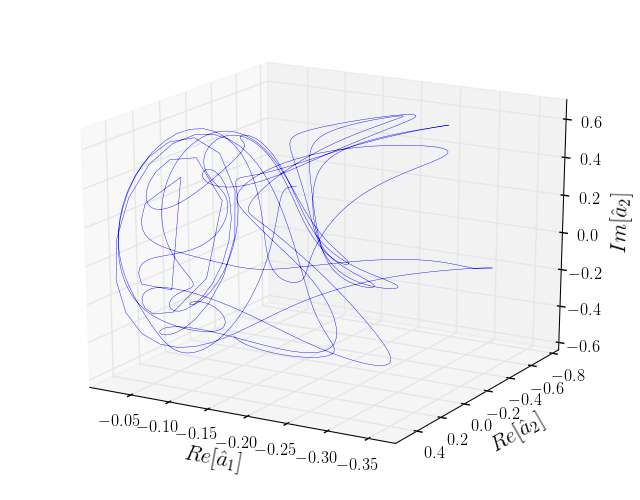
\includegraphics[width=0.9\textwidth]{BBKSmovframes}
\end{center}
\caption{ Symmetry reduced \KS\ flow . }
\label{fig:BBKSmovframes}
\end{figure}

\end{description}
\renewcommand{\ssp}{a}
